\documentclass{article}

% if you need to pass options to natbib, use, e.g.:
% \PassOptionsToPackage{numbers, compress}{natbib}
% before loading nips_2017
%
% to avoid loading the natbib package, add option nonatbib:
% \usepackage[nonatbib]{nips_2017}

% to anonymize authors, use the following and not the [final] variant
%\usepackage{nips_2017}

% to compile a camera-ready version, add the [final] option, e.g.:
\usepackage[final]{nips_2017}
\usepackage{shortcuts}
\usepackage{amsmath}

\usepackage[utf8]{inputenc} % allow utf-8 input
\usepackage[T1]{fontenc}    % use 8-bit T1 fonts
\usepackage{hyperref}       % hyperlinks
\usepackage{url}            % simple URL typesetting
\usepackage{booktabs}       % professional-quality tables
\usepackage{amsfonts}       % blackboard math symbols
\usepackage{nicefrac}       % compact symbols for 1/2, etc.
\usepackage{microtype}      % microtypography
\usepackage{color}          % color text. Using for TODO and comments.
\usepackage{listings}
\usepackage{graphicx}
\usepackage{float}

\title{Scaling Probabilistic Soft Logic for Entity Resolution}

% The \author macro works with any number of authors. There are two
% commands used to separate the names and addresses of multiple
% authors: \And and \AND.
%
% Using \And between authors leaves it to LaTeX to determine where to
% break the lines. Using \AND forces a line break at that point. So,
% if LaTeX puts 3 of 4 authors names on the first line, and the last
% on the second line, try using \AND instead of \And before the third
% author name.

\author{
  Eriq Augustine \\
  University of California, Santa Cruz\\
  1156 High St\\
  Santa Cruz, CA 95064\\
  \texttt{eaugusti@ucsc.edu} \\
  %% examples of more authors
\And
 Nikhil Kini \thanks{Equal authorship} \\
 University of California, Santa Cruz\\
 1156 High St\\
 Santa Cruz, CA 95064\\
 \texttt{nkini@ucsc.edu} \\
  %% \AND
  %% Coauthor \\
  %% Affiliation \\
  %% Address \\
  %% \texttt{email} \\
  %% \And
  %% Coauthor \\
  %% Affiliation \\
  %% Address \\
  %% \texttt{email} \\
  %% \And
  %% Coauthor \\
  %% Affiliation \\
  %% Address \\
  %% \texttt{email} \\
}

\begin{document}
% \nipsfinalcopy is no longer used

\maketitle

\section{Problem Statement}
  Probabilistic Soft Logic (PSL) is a statistical relational learning framework that aims to simplify and unify the machine learning goals of modeling richly structured data and scaling to big data. PSL scales linearly with the number of groundings. However, depending on the model rules, a  na\"{\i}ve entity resolution (ER) implementation in PSL performs a cross product of all possible assignments to the random variables in the rules. This results in space complexity that is polynomial in the number of random variable values in a rule, making it difficult to process a dataset on a single machine due to disk or memory insufficiency. The MAP inference algorithm in PSL already uses consensus optimization, which lends itself well to parallelization. However, distributing the dataset across computers requires a non-trivial partitioning of data that balances the size of the partitions and preserves the relational edges in the data. Blocking is a technique used in ER to restrict the number of comparisons to make based on some shared attribute or similarity metric. We study the scalability of PSL in an ER setting, comparing data partitioning/clustering techniques such as standard, iterative and adaptive blocking.

 TODO(eriq): Description of ADMM.

\section{Approach}

We run a number of PSL models (described below) on distributed and non-distributed systems. Towards using the distributed systems variant, we will create a custom ADMM implementation for use within PSL. Distribution naturally requires partitioning the data, and as a means of partitioning, we will implement blocking algorithms available in ER/Record Linkage literature.

Entity Resolution is commonly modeled as a binary classification problem, comparing pairs of references and classifying them as being either the same or different entities. In such a setting, comparing every pair of references quickly becomes infeasible as the number of references grows. Blocking is the term used to describe partitioning the data into subsets, called ``blocks'', such that the number of comparisons is limited to pairs of references within a block. In other words, a computationally cheap heuristic is used for preprocessing a set of potential matches. For example, suppose the entity resolution problem is to resolve academic publications in two databases. Rather than comparing every record in database 1 with every record in database 2, one can compare only those records for which the year of publication matches.  Several schemes for blocking have been proposed in the past: Standard blocking \cite{jaro1989advances} blocks references based on their sharing some chosen key, iterative blocking \cite{whang2009entity} and canopies \cite{mccallum2000efficient}, and adaptive blocking \cite{bilenko2006adaptive} which learns a blocking function dependent on the features. Blocking is very domain dependent, and not all kinds of blocking will perform well with all kinds of datasets.

Once we have our blocks, we will assign them to nodes in the cluster. Note that generally, we will have more blocks than nodes in our cluster, and hence an optimal assignment of blocks to nodes is a discrete-knapsack style NP-Complete problem. Also, note that blocks may or may not overlap in the references that they contain. Regardless, there will need to be message passing between the nodes for ADMM to reach a consensus. 

\subsection{Task(s)}

Our goal is to scale PSL to handle large datasets that require models that exhibit the cross-product behavior we see in the ER domain. Scaling can be achieved through the horizontal distribution of data and computation, and through blocking. We postulate that the efficiency of distribution might be dependent on the blocking scheme chosen. These are the questions that our project aims to answer:
\begin{itemize}
    \item Precision, recall and accuracy kept constant, is Distributed PSL faster than single node PSL?
    \item If yes, can some blocking schemes provide better speed up compared to others?
\end{itemize}

ADMM was introduced as an efficient convex optimization technique by \cite{glowinski1975approximation} and \cite{gabay1976dual}, and popularized recently as being well suited to distributed convex optimization by \cite{boyd2011distributed}. The current implementation of PSL uses ADMM for MAP inference (\cite{bach2015hinge} \S 5), and is inherently single-computer parallelizable using threads. We propose implementing distribution across several computers as a core PSL capability.

This being our main task, we describe the auxiliary tasks that PSL will perform so that we can determine those answers as follows:

We use two kinds of datasets: bibliographic data, and web log data. The task PSL will perform when applied to bibliographic data is matching entities in one database of academic papers to another database of academic papers. Entities in this context can be publication titles, authors and venues. The task PSL will perform when applied to web log data is determining whether two cookies refer to the same underlying login id. We have attributes such as IP address, GeoLocation, User Agent strings, etc. for use in our web log ER model.

For unit tests, we have also have some toy friendship data, where given observed similarities between entities, we want to predict whether they are friends. Note that this is not an entity resolution problem, and is for the purpose of testing distribution and blocking only.


\subsection{Models} \label{models}

Since our focus is scaling, we keep our model constant and vary the blocking criterion.

For the bibliographic data, our entities are publications (P) and authors (A), and our model is as follows:
\begin{eqnarray}
	\begin{aligned}
	    %if publication titles are similar -> the publications are the same
        & \pslpred{Block}(\pslarg{P1}, \pslarg{B}) \psland \pslpred{Block}(\pslarg{P2}, \pslarg{B}) \psland \pslpred{SimTitle}(\pslarg{P1},\pslarg{P2}) \implies \pslpred{SamePub}(\pslarg{P1},\pslarg{P2})\\ \nonumber
        % if authors are the same -> the publications are the same
        & \pslpred{Block}(\pslarg{P1}, \pslarg{B}) \psland \pslpred{Block}(\pslarg{P2}, \pslarg{B}) \psland \pslpred{SameAuthor}(\pslarg{P1},\pslarg{P2}) \implies \pslpred{SamePub}(\pslarg{P1},\pslarg{P2})\\ \nonumber
        % if author names are similar -> the authors are the same
        & \pslpred{Block}(\pslarg{A1}, \pslarg{B}) \psland \pslpred{Block}(\pslarg{A2}, \pslarg{B}) \psland \pslpred{SimName}(\pslarg{A1},\pslarg{A2}) \implies \pslpred{SameAuthor}(\pslarg{A1},\pslarg{A2})\\ \nonumber
        % if (author1 is coauthor with author2) and (author2 is coauthor with author3) and (author1 and author3's names are similar) -> author1 and author2 are the same
        & \pslpred{Block}(\pslarg{A1}, \pslarg{B}) \psland \pslpred{Block}(\pslarg{A2}, \pslarg{B})  \psland \pslpred{Block}(\pslarg{A3}, \pslarg{B}) \\ \nonumber 
        & \ \ \ \  \psland  \pslpred{CoAuthors}(\pslarg{A1}, \pslarg{A2}) \psland \pslpred{CoAuthors}(\pslarg{A2}, \pslarg{A3}) \implies \pslpred{SameAuthor}(\pslarg{A1},\pslarg{A3})  \\ \nonumber
        % Author transitivity
        & \pslpred{Block}(\pslarg{A1}, \pslarg{B}) \psland \pslpred{Block}(\pslarg{A2}, \pslarg{B})  \psland \pslpred{Block}(\pslarg{A3}, \pslarg{B}) \\ \nonumber 
        & \ \ \ \  \psland  \pslpred{SameAuthor}(\pslarg{A1}, \pslarg{A2}) \psland \pslpred{SameAuthor}(\pslarg{A2}, \pslarg{A3}) 
        \implies \pslpred{SameAuthor}(\pslarg{A1},\pslarg{A3}) 
	\end{aligned}
\end{eqnarray}

For the web log data, our entities are logged in users who often have several cookies (C) for the same website, usually across several devices. The model is as follows:
\begin{eqnarray}
	\begin{aligned}
	    %Negative prior
        & \pslpred{Block}(\pslarg{C1}, \pslarg{B}) \psland \pslpred{Block}(\pslarg{C2}, \pslarg{B}) \implies \pslneg \pslpred{Same}(\pslarg{C1},\pslarg{C2})\\ \nonumber
	    %Similarity
        & \pslpred{Block}(\pslarg{C1}, \pslarg{B}) \psland \pslpred{Block}(\pslarg{C2}, \pslarg{B}) \psland \pslpred{Sim}(\pslarg{C1},\pslarg{C2}) \implies \pslpred{SameUser}(\pslarg{C1},\pslarg{C2})\\ \nonumber
        %Transitivity
        & \pslpred{Block}(\pslarg{C1}, \pslarg{B}) \psland \pslpred{Block}(\pslarg{C2}, \pslarg{B}) \psland \pslpred{SameUser}(\pslarg{C1},\pslarg{C2})  \\ \nonumber
        & \ \ \ \ \psland \pslpred{SameUser}(\pslarg{C1},\pslarg{C2}) \psland (\pslarg{C1} \neq \pslarg{C3}) \implies \pslpred{Same}(\pslarg{C1},\pslarg{C3})
	\end{aligned}
\end{eqnarray}

The coauthor rule is relational in the bibliography ER model and the relational rule used in the web log model is the transitivity rule.

Note that the predicate \pslpred{Sim} in the web log model combines the similarity of various attributes of the data. For instance, similarity between two cookies can be computed by combining the similarity of IP addresses, User agents and Geographic information. Similarly (no pun intended), the similarity metrics used in the bibliograhy model for the predicates \pslpred{SimTitle} and \pslpred{SimName} is a choice to exercise. The \pslpred{Block} predicates are computed by using one of many possible blocking schemes.

\subsection{Evaluation}

In terms of comparisons, we mainly want to compare the runtimes of distributed PSL and single node PSL, and the reduction ratio and recall metrics for the blocking techniques.

The runtimes will change compared to single machine PSL because of the overhead of distribution and the additional computational cores available. However, it should be noted that much larger problems can now be solved because of the increase in available memory.

Precision and recall will vary on account of blocking. Blocking introduces a trade-off between recall and compression. (1.0 - Recall) is the cost of blocking, because blocking can result in references to the same entity never getting matched. Compression, known better as ``reduction ratio'' in ER, is the percentage of comparisons saved due to blocking. 

Formats for evaluation are spelled out in the Section \ref{proposed_eval}.
%We will use existing ER systems from literature that have used the bibliographic dataset as comparisons. We also propose to compare Felix \cite{niu2011scaling}, a distributed MLN system, with distributed PSL. We would also like to see the effects of Compression and recall on the runtimes and precision-recall.

\section{Data}

The entity resolution literature has several often-used bibliographic datasets, used especially in the study of blocking techniques. A benefit of this data is the wealth of existing comparisons. The database group Leipzig hosts some bibliographic ER datasets \cite{kopcke2010evaluation}. \url{https://dbs.uni-leipzig.de/en/research/projects/object_matching/fever/benchmark_datasets_for_entity_resolution}. 

Details about the datasets are on this page \href{https://dbs.uni-leipzig.de/de/research/projects/object_matching/fever/benchmark_datasets_for_entity_resolution}{page}\footnote{\url{https://dbs.uni-leipzig.de/de/research/projects/object_matching/fever/benchmark_datasets_for_entity_resolution}}. There are four datasets from this group -- two bibliographic and two e-commerce. Each dataset is comprised of two different databases (simple, single table), of possibly the same entities (academic paper or shopping product), so that the entity resolution problem manifests as a record linkage problem. The attributes are \{title, authors, venue, year\} for the bibliographic databases, and \{name, description, manufacturer, price\} for the E-commerce databases. Some observations about the datasets:
\begin{itemize}
    \item Overall impression: These are decent datasets for testing, but certainly too small for any scalability experiments. They're also less clean than we'd like them to be.
    \item Missing / incorrect data: The Scholar database in the DBLP-Scholar dataset has over 50\% records missing their year field, and some have incorrect years like 0, 20, 2703. We think this explains the poor recall. Similarly, in the Amzn-Goog dataset, under 10\% of the Goog database has a value for manufacturer. The Abt database in the Abt-Buy dataset is missing the manufacturer attribute completely. We improvised a column noticing that the first word of the name field in the record was consistently the brand/manufacturer.
    \item Limited range: The bibliographic data seems to be limited to about ten years and a handful of venues only.
    \item The most important problem with these bibliography datasets is that they only provide ground truth for the publication titles, and not for authors. Post-processing for matching authors will certainly lead to some noise.
\end{itemize}

We also want to use real-world data in the form of cross-device visitor web logs, courtesy of Adobe Systems Inc. Adobe's data contains web log entries of visits to a media website collected over 20 days. Not all visitors signed into their account for their web sessions. Each visit is a mention and is identified by a cookie ID. The portion of these visits that logged in comprise the ground truth entity labels. That is, each individual entity is identified by a login ID. The ER problem is mapping the cookie IDs to the corresponding login IDs. Note that there can be several cookie IDs associated with a login IDs, which makes it an ER problem; but it is made challenging by the fact that such multi-cookie logins constitute a very small portion of the dataset. Some statistics:
    \begin{itemize}
        \item Mean number of cookies $\approx$ 1.4million
        \item Mean number of login IDs = 10443
        \item Mean number of login IDs with 2 or more cookies = 1392
    \end{itemize}
    
The mean is over 10 partitions of the dataset, where partitioning ensured that there was no overlap of cookies and login IDs. There are around 70 such partitions, but we use 10 for now. The partitions are good for use for cross-validation. 

Both these domains carry at least some relational information. These are leveraged in the rules written in the models in Section \ref{models}. Transitivity is easily applied to the web log data, but is not usable when linking records in two separate databases, which is the case with bibliographic data.


\section{Baselines}

We present two baselines: one baseline for blocking, and another for runtimes. The baseline for blocking is standard blocking, which blocks on a matching attribute. The baseline for runtime is inference time for PSL run on a single node. These baselines will be compared against more advanced blocking techniques and against the runtime for PSL run on multiple nodes, respectively.

\subsection{Blocking baseline}

We present results of applying standard blocking on the Database Group Leipzig ER datasets in Table \ref{table:stdblock-leipzig}. Of interest to us are the first two rows, the bibliographic datasets. We see that blocking by year results in total recall for the DBLP-ACM dataset, while it fares quite poorly (less that 50\%) when used with DBLP-Scholar. An underlying reason for this is that the Scholar database is machine-extracted with little human curation (at the time of the creation of this dataset) which results in several errors and omissions in the attributes.

%TODO (Nikhil) make a table out of this, with statistics about other blocking keys like IP Address and user agent
For the Web Log dataset, we have the following statistics with blocking done on a GeoLocational attribute called `region':\\
Num comparisons without blocking $\approx$ 1 trillion (1,045,110,265,920 to be exact)\\
Num comparisons after blocking $\approx$ 19 billion (19,358,182,888 to be exact)\\
Compression: 98.15\%\\
Recall: 96.70\%

Despite 98\% compression, we are still left with 19 billion comparisons. Both these baselines show a clear motivation for better blocking techniques, as well as for distributing grounding and computation across nodes to handle the scale.

\begin{table}
\centering
\begin{tabular}{*{10}{l}}  
\toprule
& \multicolumn{2}{c}{\#Mentions} & &   & &       \multicolumn{2}{c}{$\approx$ \#comparisons}    &  &    \\
\cmidrule(r){2-3} \cmidrule(r){7-8}
Name     & DB1  & DB2 &  \#True & Key & \#Blocks & Before  & After  & Recall & Compr. \\
\midrule
%DBLP-ACM & 2616 & 2294 & 2224        & Year     & 11       & 3000552 & 300642 & 0.8998 & 1.0      \\
%DBLP-Scholar & 2616 & 64263 & 5347   & Year     & 128      & 84056004 & 2133744 & 0.4533 & 0.9746      \\
%AMZN-GOOG & 1363 & 3226 & 1300 & Manuf. & 381 & 2198519 & 916 & 0.0254 & 0.9996    \\
%Abt-Buy & 1081 & 1092 & 1097    & Manuf.  & 162   & 590226 & 28768 & 0.7703 & 0.9513      \\
DBLP-ACM & 2616 & 2294 & 2224        & Year     & 11       & 3m & 300k & 1.0 & 0.8998 \\
DBLP-Scholar & 2616 & 64263 & 5347   & Year     & 128      & 84m & 2.1m & 0.4533 & 0.9746 \\
Amzn-Goog & 1363 & 3226 & 1300 & Manuf. & 381 & 2.2m & 916 & 0.0254 & 0.9996    \\
Abt-Buy & 1081 & 1092 & 1097   & Manuf. & 162 & 590k & 29k & 0.7703 & 0.9513 \\
\bottomrule
\end{tabular}
\caption{Statistics for the four Leipzig datasets, with results for standard blocking. Key is the attribute used for blocking, \#True is the number of ground truth pairs in the dataset.}
\label{table:stdblock-leipzig}
\end{table}

\subsection{Runtime Baseline}

To compare the performance of our distributed implementation of ADMM/PSL in a controlled fashion, we have constructed a synthetic data generator to test on.
The goal of this dataset is to predict friendship links given some information about a person.

Our model contains the following information:
\begin{itemize}
    \item \textbf{Similar} - A random similarity measure between two people. This can represent the aggregation of the similarity of several local features.
    \item \textbf{Friends} - The target data that we are trying to predict. We will try to infer the friendship on the full cross-product of people.
    \item \textbf{Location} - An arbitrary location that people are assigned to.
\end{itemize}

Both the number of people and number of locations are parameters that we can tune.
People in different locations are placed into different blocks.
Each block is then allocated to a worker node in our cluster.

We define the following PSL rules on this data:
\begin{eqnarray}
	\begin{aligned}
        & \pslpred{Block}(\pslarg{P1}, \pslarg{B}) \psland \pslpred{Block}(\pslarg{P2}, \pslarg{B}) \psland (\pslarg{P1} \neq \pslarg{P2}) \psland \pslpred{Similar}(\pslarg{P1}, \pslarg{P2}) & \implies \pslpred{Friends}(\pslarg{P1}, \pslarg{P2}) \\ \nonumber
        & \pslpred{Block}(\pslarg{P1}, \pslarg{B}) \psland \pslpred{Block}(\pslarg{P2}, \pslarg{B}) \psland \pslpred{Block}(\pslarg{P3}, \pslarg{B}) \\ \nonumber 
        & \ \ \ \ \ \ \ \ \ \ \ \ \ \ \ \ \ \ \  \psland (\pslarg{P1} \neq \pslarg{P3}) \psland  \pslpred{Friends}(\pslarg{P1}, \pslarg{P2}) \psland \pslpred{Friends}(\pslarg{P2}, \pslarg{P3}) & \implies \pslpred{Friends}(\pslarg{P1}, \pslarg{P3})  \\ \nonumber
        & \pslpred{Block}(\pslarg{P1}, \pslarg{B}) \psland \pslpred{Block}(\pslarg{P2}, \pslarg{B}) \psland (\pslarg{P1} \neq \pslarg{P2}) \psland \pslpred{Friends}(\pslarg{P1}, \pslarg{P2}) & \implies \pslpred{Friends}(\pslarg{P2}, \pslarg{P1})
    \end{aligned}
\end{eqnarray}

Our model states three things:
\begin{enumerate}
    \item Similar people are likely to be friends
    \item Friendship is transitive
    \item Friendship is symmetric
\end{enumerate}

Our data and model are simple, but the friendship crossproduct, symmetry, and transitivity quickly generate an exponential number of ground rules.
Table \ref{tab:synthetic-runtimes} shows the results of a distributed PSL clusters versus a standalone PSL instance on the synthetic data.
%TODO (Eriq) - but it didn't for the 20 people sized expt according to the table, no?
Note that the distributed PSL beat out the standalone PSL on all versions of this synthetic dataset.
\footnote{All runs achieved the same accuracy.}

%TODO (Eriq) 
% a) are these results statistically significant? Typical you want to report the average runtime of about 10 runs.
% b) perhaps information about number of groundings might be a useful column in this table?
\begin{table}
   \begin{center}
      \begin{tabular}{| c | c | c | c |}
         \hline
            People & Locations & Cluster Size & Inference Runtime (ms) \\
         \hline
            20 & 3 & 1 & 849 \\
            20 & 3 & 2 & 1020 \\
            100 & 3 & 1 & 11200 \\
            100 & 3 & 2 & 7701 \\
         \hline
      \end{tabular}
      \caption{Runtimes on synthetic data.}
      \label{tab:synthetic-runtimes}
   \end{center}
\end{table}


\section{Experiments}

A recap of our goals:

Large problems do not fit on single node machines on account of the memory requirements for grounding rules. Under blocking scheme 1, we expect <TODO> number of ground rules, and we were not able to fit this on the largest server available to us with 384GB of RAM.

To overcome this limitation, we propose that the grounding of rules be distributed across several nodes. In an entity resolution problem, the need for blocking to reduce the number of comparisons naturally offers a partitioning scheme. Under this scheme, nodes are assigned blocks and each node only grounds the rules corresponding to the blocks that it is assigned, thereby reducing the number of ground rules per node. TODO: show a graph or table of the reduction in groundings per node?

A reminder of the problem size: We have 1295 publication mentions of 134 distinct publications, and 3524 author mentions of 51 distinct authors.

Not all blocking schemes are equal, especially in the context of their use in partitioning data. In our na\"{\i}ve author blocking scheme BM1, we create a set $s_i$ of the first character of each token in an author's mention $m_i$. Each such set is used as a blocking key. A mention is assigned to a block if its set of first characters are a subset of or equal to the blocking key. Then, a mention $m_{i_1}$ and a mention $m_{i_2}$ are in the same block if $s_{i_1} \cap s_{i_2} \neq \emptyset$. This results in 80 blocks, with a mean of 86 mentions, and a standard deviations of 156. Five blocks have over 500 elements, and since a block is the minimum unit of data partitioning, the problem of insufficient memory manifests when these 500+ element blocks are assigned to some machine, especially with the transitive rule. Hence we prefer blocking schemes that result in smaller block sizes.

To take advantage of the relational nature our model, and the nature of author mentions in citations where there are several exactly matching overlaps, we design a two-level hierarchical blocking scheme. The first level of blocks are based on string equality. Two mentions are in the same block if they match exactly. This results in 189 block keys (from 3524 mentions), $bk1_1, bk1_2, ... bk1_324$. The second level of blocking creates a blocking key $bk2_j$ using the same BM1 criterion as above, conceptually operating on the block keys $bk1_i$ rather than the mentions. If $bk1_{i_1}$ and $bk1_{i_2}$ have the same $bk2_j$, a small percentage $\eta$ of mentions from each $bk1_i$ are added under the block.

$\eta$ is a parameter that allows us to control the size of the blocks at level two, and also control the recall and reduction ratio as measured in a non-hierarchical setting. Our hypothesis is that even with a small percentage of eta, using a relational model will enable us to recover the entity matches across the $bk2$ hierarchical level.

Some discussion about blocking methods:

Blocking methods used, all for blocking author mentions. Remember, it needs to be inexpensive to compare. We started with some na\"{\i}ve methods:

$C_3$ is the set of upto 3 characters from each token in the mention.
% Code: dfauthors['blockcondition1_3letters'] = dfauthors['name'].apply(lambda x : set([part_of_name.replace('.','')[:3] for part_of_name in x.split(' ')]))

$I$ is the set of the first character from each token in the mention.
% Code: dfauthors['blockcondition2_sortedInitials'] = dfauthors['name'].apply(lambda x : ''.join(sorted([part_of_name[0] for part_of_name in x.replace('.','').split(' ') if part_of_name !=''])))

Two mentions are in the same block if

\begin{itemize}
    \item The intersection of their $C_3$ has at least two elements
    \item The intersection of their $C_3$ has at least one element
    \item The intersection of their $C_3$ has at least one 3 character element
    \item The intersection of $I$ of one mention is a subset of the other mention
\end{itemize}


We also implemented and tested the following more advanced methods: Adaptive blocking (\cite{bilenko2006adaptive}) and Canopies (\cite{mccallum2000efficient}).

In our goal for more efficient distribution, and to exploit the relational nature of PSL, we implemented a two-level hierarchy blocking scheme with a distribution parameter $\eta$.

\begin{table}
   \begin{center}
      \begin{tabular}{| c | c | c | c | c |}
         \hline
            Blocking Method & Compression & Recall & Number of blocks & ($\mu, \sigma$) mentions per block \\
         \hline
             & & & &  \\
             & & & &  \\
             & & & &  \\
             & & & &  \\
         \hline
      \end{tabular}
      \caption{Comparison of blocking techniques}
      \label{tab:blocking-stats-compare}
   \end{center}
\end{table}


Some discussion about the choice of similarity:

The similarity metric chosen plays a vital role in the results, as we observed in one of our experiments. We started with using Jaro-Winkler distance for both, publication titles and author mentions. However, we saw poor precision (0.1871) with our model. However, changing to cosine similarity on TF-IDF vectorized publication titles improved the precision to 0.9589, a jump with no other changes to the model. This improvement did come at the cost of reduced recall, which went down from 0.8579 to 0.7955. We refrain from further improving our model, since our goal for this project is scalability. We do however, intend to tune the model and formally learn weights in the future.


\section{Proposed Evaluation} \label{proposed_eval}

\begin{figure}[htb!]
    \centering
    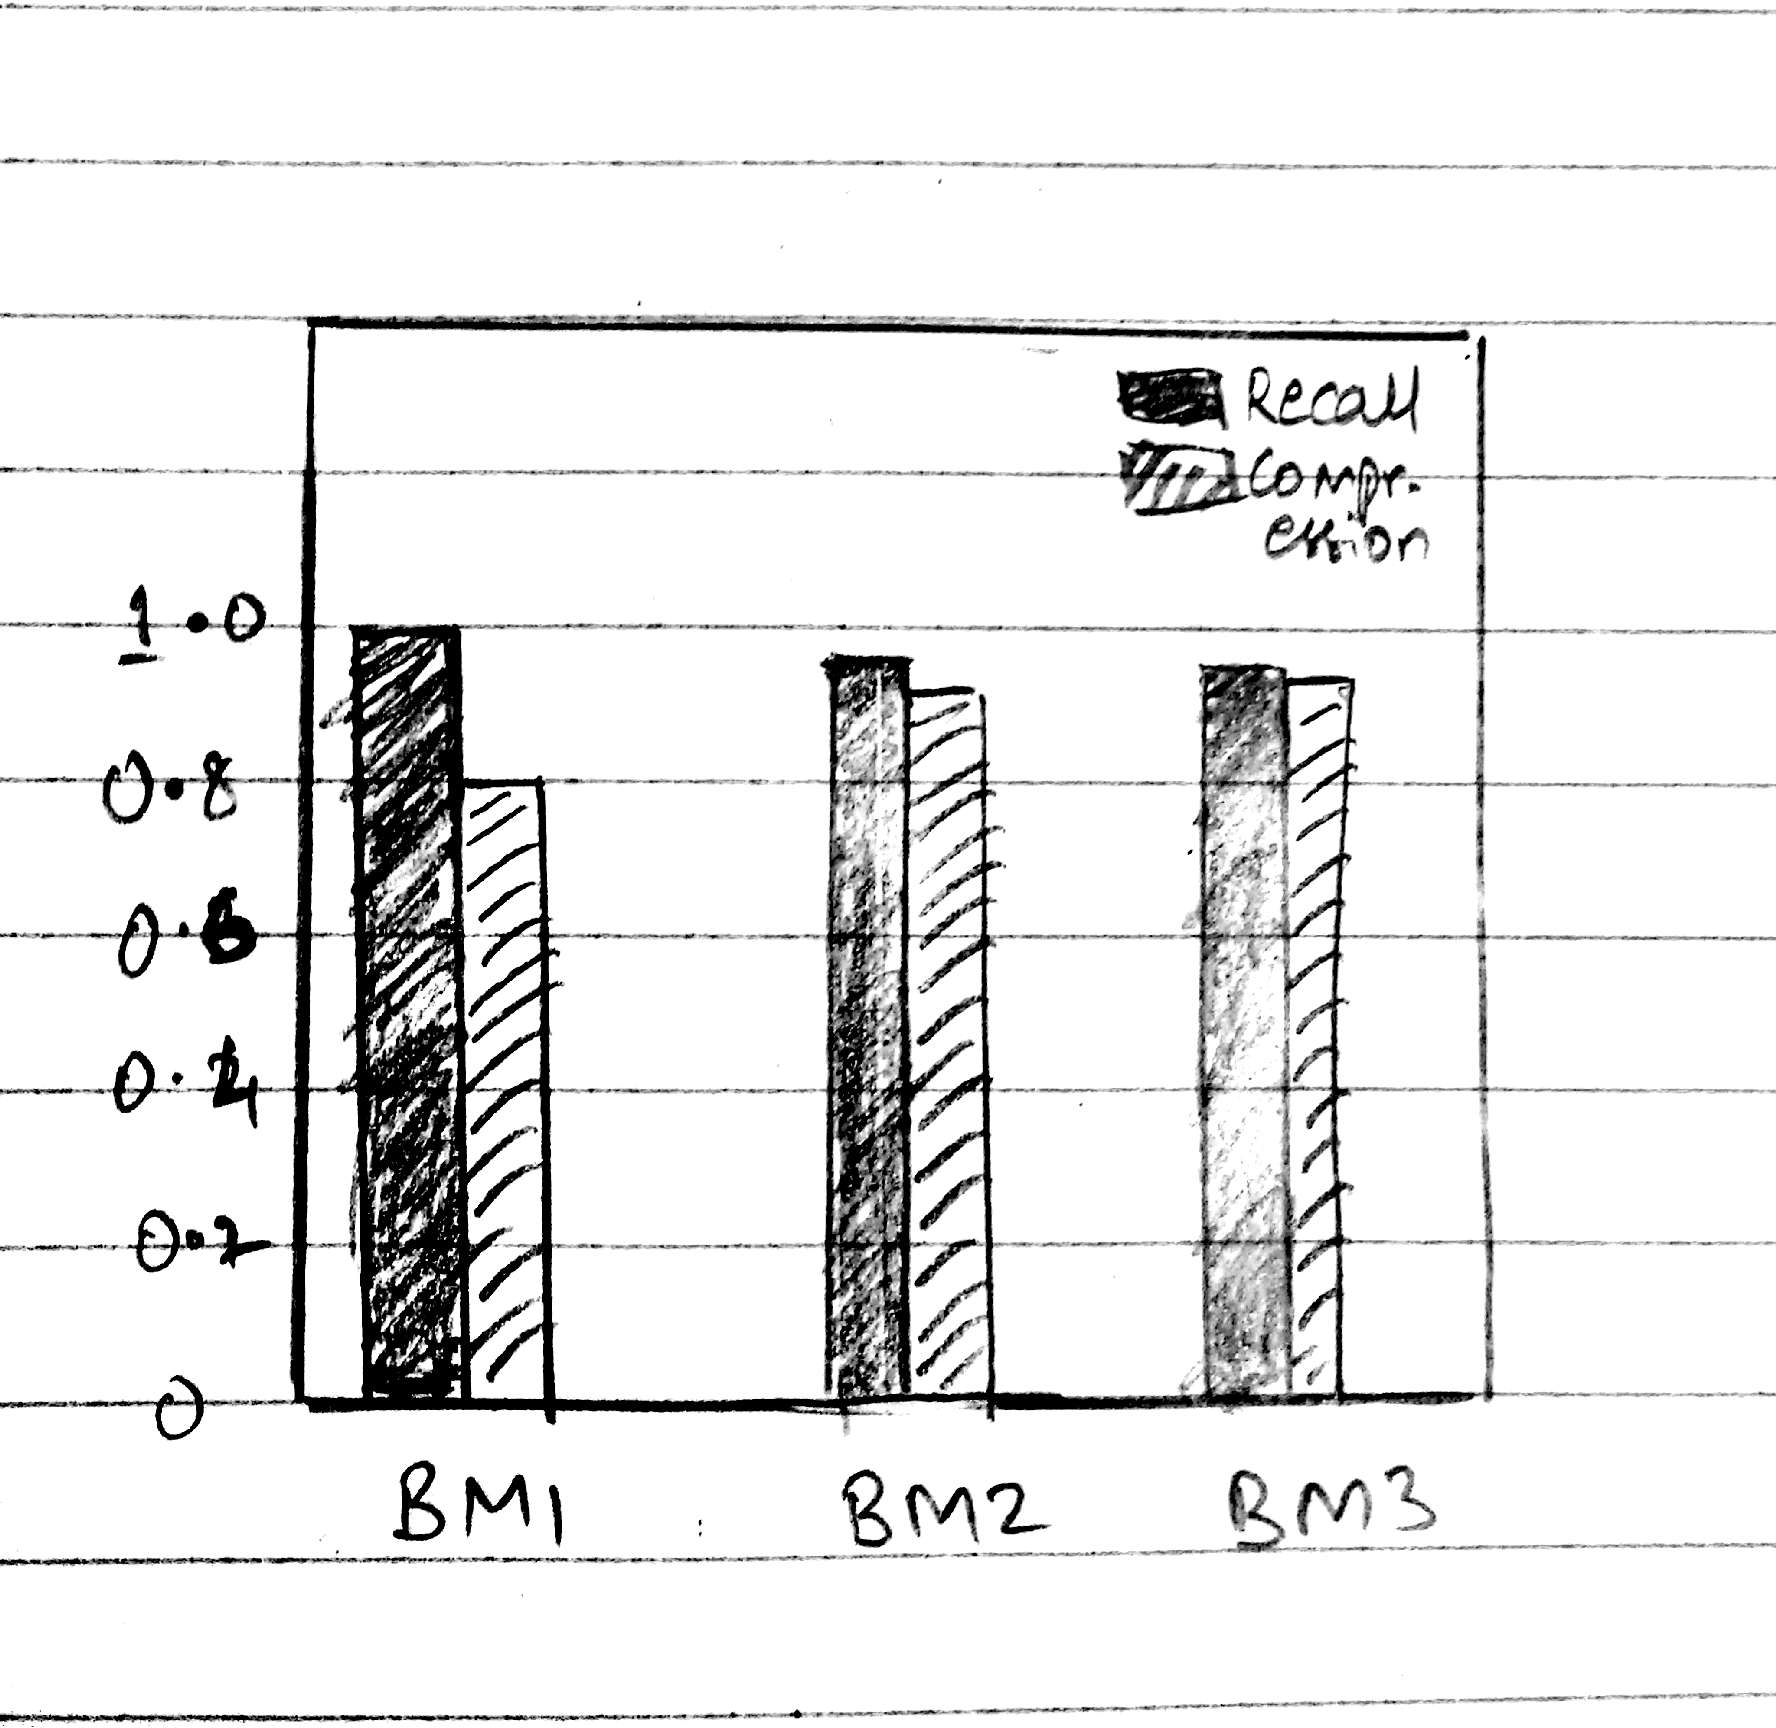
\includegraphics[width=0.53\textwidth]{BM-RecComp}
    \caption{A comparison of the blocking methods based on their Recall and Compression}
    \label{fig:reccomp}
\end{figure}

\begin{figure}[htb!]
    \centering
    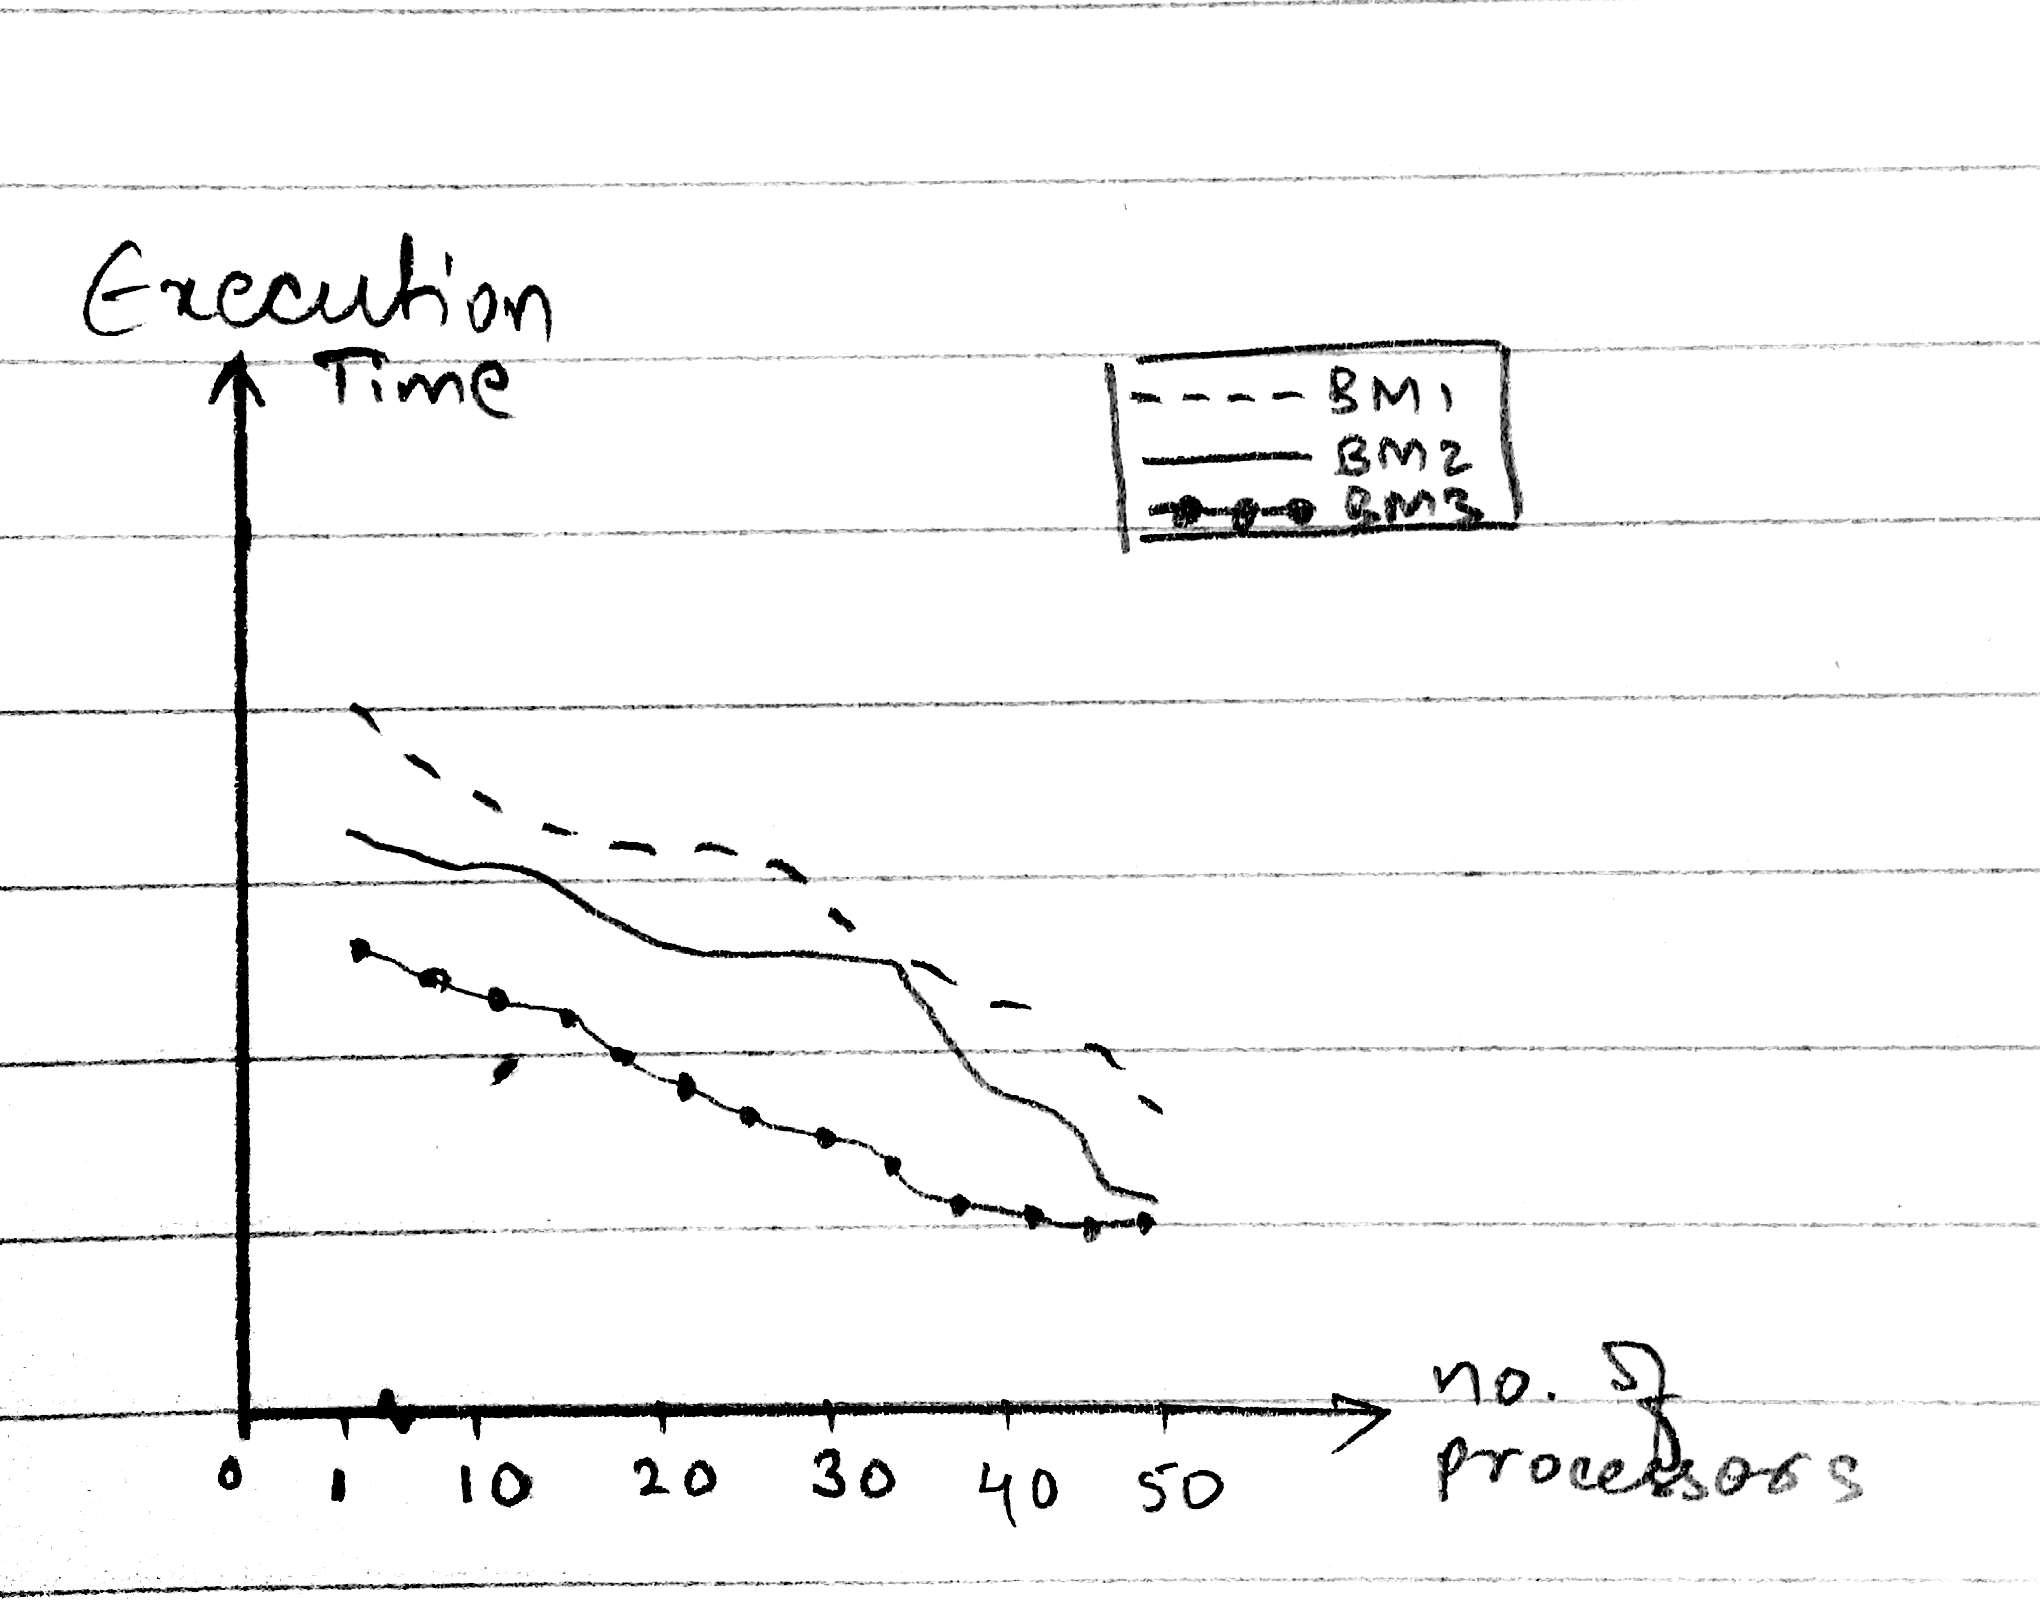
\includegraphics[width=0.53\textwidth]{NumProcvsRuntime}
    \caption{A comparison of the runtime  as the number of processors (equivalently, nodes) varies}
    \label{fig:numproc}
\end{figure}

\begin{figure}[htb!]
    \centering
    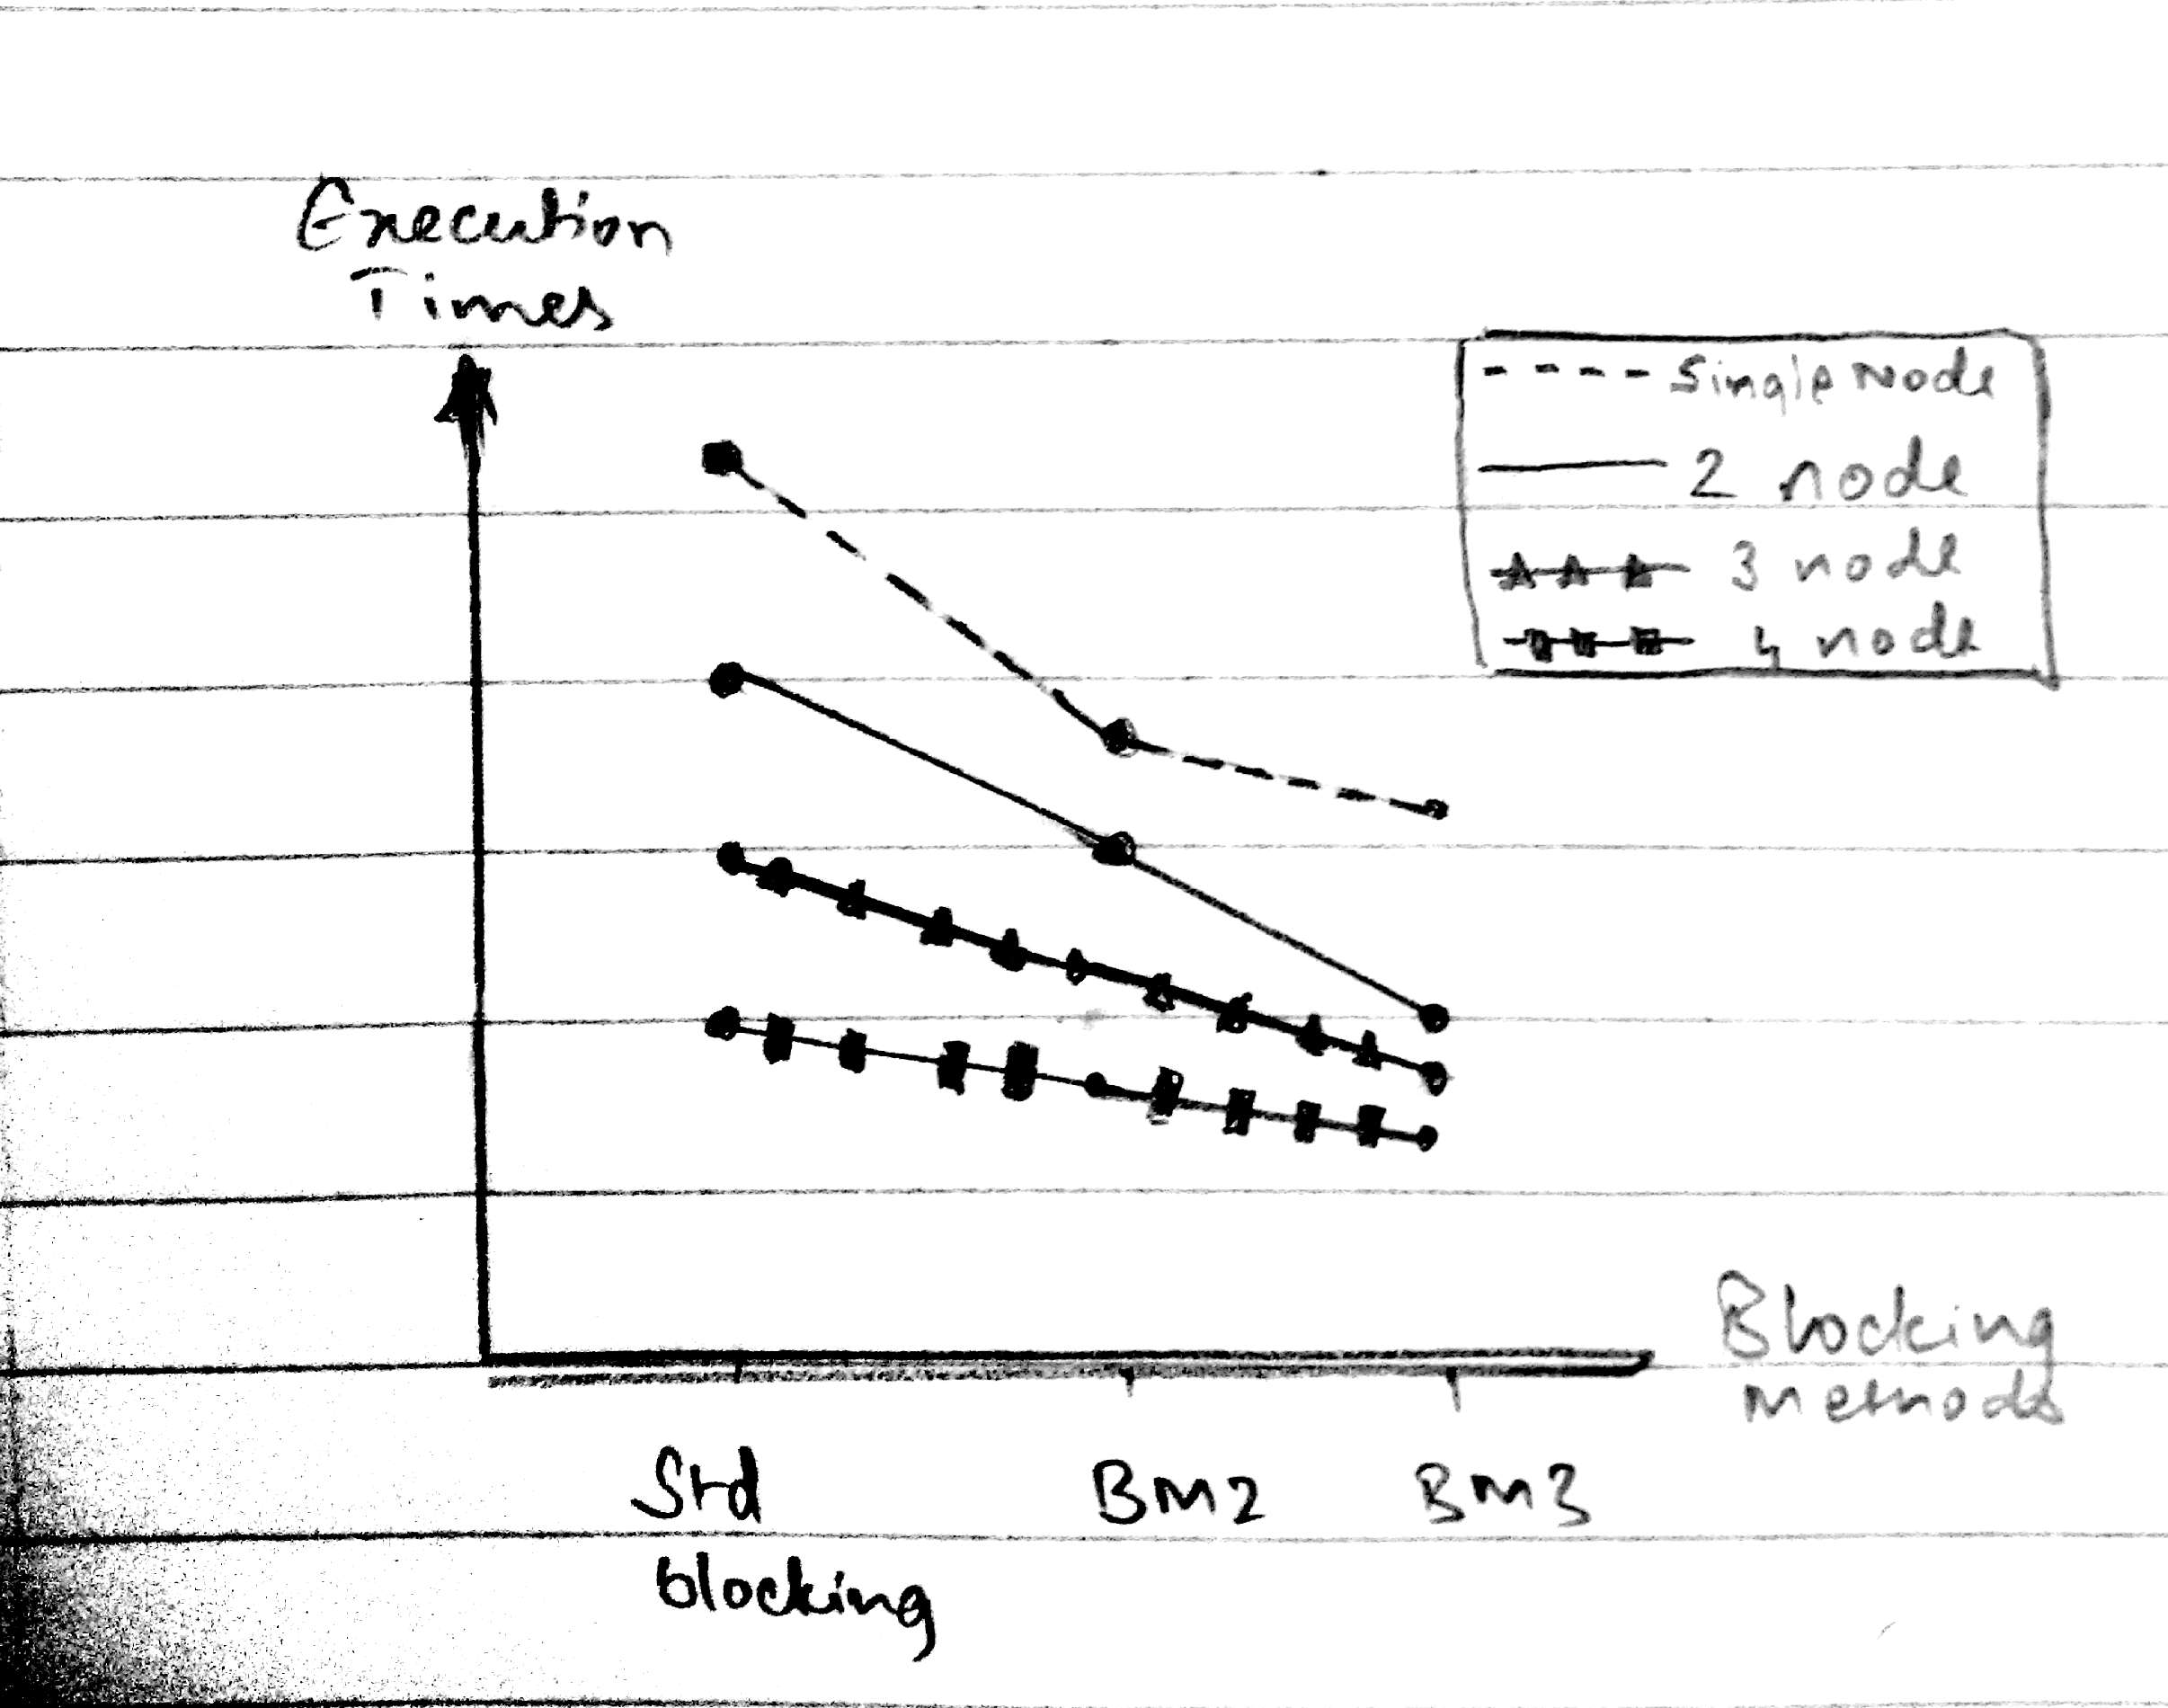
\includegraphics[width=0.53\textwidth]{BMvsRuntime}
    \caption{Do blocking methods affect distributed performance?}
    \label{fig:bmruntime}
\end{figure}

This sections lists some ideas about how we would like to present our results. Feedback will be greatly appreciated. IMPORTANT: THESE ARE FAKE PLOTS/TABLES, meant to only be illustrative of our proposed template of presentation.

\section{Related work}

\subsection{Entity resolution}

Statistical relational techniques have been previously applied to entity resolution. Notably, \cite{singla2006entity} address Entity Resolution using Markov Logic Networks.  \cite{bhattacharya:thesis06} predates PSL, contains important work about formulating ER as a collective inference problem. It compares several similarity and neighbourhood similarity metrics, and introduces a relational clustering algorithm. For a more recent treatment, albeit within the context of knowledge graph ER, \cite{pujara:starai16} describes common modeling patterns and rules.

\cite{kopcke2010frameworks} provide a nice overview of several entity resolution solutions. We use the same bibliographic datasets that they use enabling a comparison with their metrics.

Distributed scaling has been successfully implemented in the past in \cite{pujara:thesis16} for knowledge graph identification (KGI), where a knowledge graph was partitioned across multiple machines. In the domain of ER, just as in the domain of KGI, the challenge lies in partitioning data without losing relationships in the graphical model.

\subsection{Parallelizing Entity Resolution}

There are several papers that specifically talk about distributing or parallelizing Entity Resolution problems. \cite{benjelloun2007d} and \cite{kawai2006p} presents a family of algorithms for distributing/parallelizing the ER workload across multiple processors. This is a family of algorithms because they treat the matching and record merging functions (as well as the distributing functions) as black boxes, where any relevant function of choice can be substituted. \cite{efthymiou2017parallel} introduces algorithms for Meta-blocking that use the MapReduce framework. Meta-blocking is used to clean the overlapping blocks from unnecessary comparisons. \cite{dal2011fast}'s MD-approach combines an efficient blocking method with a robust data parallel programming model for a scalable deduplication solution. \cite{malhotra2014graph} compare two distribution approaches that they call bucket-centric and record-centric with a focus on load balancing. \cite{kirsten2010data} propose different strategies to partition the input data and generate multiple match tasks that can be independently executed. \cite{kim2007parallel} study scenarios where the collections being compared/merged are clean, only one is clean, and both are dirty to exploit interplay between match and merge to achieve parallelization. \cite{rastogi2011large} propose a principled framework to scale any generic entity matching algorithm by running multiple instances of the EM algorithm on small neighborhoods of the data and passing messages across neighborhoods to construct a global solution.

For some reference code, there are the following open-source implementations of distributed ADMM:
\begin{itemize}
    \item Hadoop Implementation of the ADMM algorithm: \url{https://github.com/intentmedia/admm}
    \item Generic Implementation of Consensus ADMM over Spark: \url{https://github.com/yahoo/SparkADMM}
\end{itemize}

There are some relevant papers that take relational information into account: \cite{Martins:2011:DDM:2145432.2145460} and \cite{aguiar2011augmented} which likely influenced the \cite{bach2012scaling} paper. While \cite{bach2012scaling} doesn't actually distribute data over multiple machines, it is more detailed in its explanation of scaling MPE inference with HL-MRFs than \cite{bach2015hinge}.

\subsubsection*{Acknowledgments}

Use unnumbered third level headings for the acknowledgments. All acknowledgments go at the end of the paper. Do not include acknowledgments in the anonymized submission, only in the final paper.

\bibliography{references} 
\bibliographystyle{apalike}

\end{document}
